% LEXICAL STRESS ERRORS
%
% !TEX root = ../thesis-main.tex
%
%TODO change title? \chapter{Lexical stress errors in the IFCASL corpus}
\chapter{Lexical stress errors by French learners of German \TODO{retitle?}}
\label{chap:lexstress}

%\cleanchapterquote{You can’t do better design with a computer, but you can speed up your work enormously.}{Wim Crouwel}{(Graphic designer and typographer)}

%\blindtext

%\section{Stress in German vs. French }
%	\subsection{Comparative prosody}
%	\subsection{Stress ``deafness'' in French}
%	\subsection{Expected errors}
%	
	
%\TODO{Change title?}
%\section{Lexical stress errors in the IFCASL corpus} 

\TODO{``sub-corpus'' gets pretty annoying in this chapter - think of better term?}

	\TODO{Recap of IFCASL corpus  \cref{sec:intro:ifcasl}}

	To investigate to what extent the expected lexical stress errors by French speakers of German are actually produced, a subset of the non-native German-language IFCASL corpus was annotated for such errors.
	\TODO{more about why this is necessary/how the corpus will be used for supervised training}
	%
	The first sections of this chapter describe the selection of material for this sub-corpus (\cref{sec:lexstress:data}), the annotators who labeled lexical stress errors in that data (\cref{sec:lexstress:annotators}), and the method by which annotation was performed (\cref{sec:lexstress:method}). 
	
	Once error judgments had been collected from each annotator, different annotators' judgments of the same utterances were compared to determine the reliability of the annotation, i.e. the agreement between annotators.
	%, which gives some indication of the general difficulty of the task of diagnosing lexical stress errors in nonnative German speech. 
	\Cref{sec:lexstress:agreement} describes this analysis of inter-annotator agreement, which aims to shed light on the following questions:
	\begin{itemize}
	\item{How reliably can lexical stress errors be identified by
	%Can lexical stress errors be reliably identified by 
	%native German speakers 
	annotators, i.e. to what extent do the judgments of different annotators agree?  (\cref{sec:agreement:overall})}
	\item{Are there differences in how native and non-native German speakers identify errors?  (\cref{sec:agreement:native})}
	\item{Are there differences in how expert and novice annotators (those without annotation experience or any training in phonetics/phonology) identify lexical stress errors?  (\cref{sec:agreement:expert})} 
	\end{itemize}
	%
	As \cref{sec:lexstress:agreement} will show, annotators did not always agree as to whether a given utterance exhibited a lexical stress error or not. Nevertheless, a ``gold-standard'' label for each utterance had to be determined; \cref{sec:agreement:gold} describes how this was accomplished in cases of disagreement.
	
	Finally, given the gold-standard labels for each utterance, the distribution of lexical stress errors in the sub-corpus was analyzed; the following questions guided this analysis, which is detailed in \cref{sec:lexstress:results}.
	\begin{itemize}
	\item{Are lexical stress errors observed frequently in the IFCASL data? (\cref{sec:results:overall})}
	\item{Is there a difference in the frequency of these errors among different groups of speakers (i.e. in terms of skill level, age, or gender) or in different contexts (e.g. after hearing a native speaker produce the word)?  (\cref{sec:results:level,sec:results:agegender,sec:results:condition})}
	\item{Are lexical stress errors observed more frequently with certain word types than with others?  (\cref{sec:results:wordtype})}
	\item{How frequently do technical problems interfere with determining whether an error was made?  (\cref{sec:results:techproblems})}
	\end{itemize}
	
	%--moved to before questions--
	%This chapter describes the annotation of this sub-corpus, and presents an analysis of the annotated data that provides tentative answers to the above questions. \TODO{rephrase that?}
	%This chapter presents the data and method used for this annotation, and an analysis of the annotated sub-corpus \TODO{\textit{rephrase}: in light of these guiding questions}.
 
	
	%\subsection{Data}
	\section{Data}
	\label{sec:lexstress:data}
	
	The IFCASL sub-corpus annotated for lexical stress errors consists of utterances of twelve word types (see \cref{tab:bisyllwords}), each of which is bisyllabic and canonically has its primary stress on the initial syllable. These characteristics were chosen deliberately: the selected words are bisyllabic because this simplifies comparison between stressed and unstressed syllables, and they are initial-stress because this is the stress pattern which native (L1) French speakers are expected to have the most difficulty producing in German, given the fixed final-position stress and final lengthening in French (see \cref{sec:stress:expected}). 
	
	In the IFCASL corpus recordings, sentences containing these words were read aloud by L1 and L2 (L1 French) speakers. Here, only the L2 utterances were annotated; it is assumed that the L1 German speakers always realize lexical stress correctly. \TODO{justify that assumption?}
	
	As described in \cref{sec:intro:ifcasl} \TODO{verify that this reference is appropriate}, the IFCASL recordings were performed under two conditions: the ``Sentence Read'' (SR) condition, in which the L2 speaker is simply  presented with the text of the sentence and asked to record themselves reading it aloud, and the ``Sentence Heard'' (SH) condition, in which the L2 speaker is asked to listen to an utterance of the sentence by an L1 German speaker before recording their own utterance. The sub-corpus for annotation includes recordings from both conditions, though the majority are from the SR condition \TODO{does mentioning that help or hurt?}.
	
	To compile the sub-corpus for annotation, utterances (tokens) of each word as produced by over 50 L2 speakers were extracted from the recordings automatically with Praat \parencite{Boersma2014}, using extraction times (start and end points of word utterances) taken from the word-level segmentation of each sentence utterance automatically obtained by forced alignment (see \cref{sec:diag:segmentation}).
	\Cref{tab:bisyllwords} lists the exact number of tokens available for each word type. In total, 669 word tokens were annotated for lexical stress errors. 
	Four tokens had to be excluded from the data, as disfluencies in the sentence utterance (e.g. false starts or repetitions of the target word) prevented the automatic extraction of the word utterance from the sentence as a whole. In a fully-fledged student-facing CAPT system, such disfluencies would need to be dealt with accordingly, e.g. by means of a pre-processing step which analyzes the student's utterance for possible disfluencies and compensates for any that are detected by, for example, prompting the student to re-record their utterance. However, detecting disfluencies in speech, especially non-native speech, is an area of active research (see e.g. \TODO{refs}), and the development of a  disfluency-aware system is outside the scope of this thesis project; therefore, this work presupposes that no disfluencies exist in the student's utterance, and the handful of disfluent tokens have been excluded from the error-annotated sub-corpus described here.
	
	\begin{table}[htb]
		\centering
		\caption{The twelve bisyllabic initial-stress words types selected from the IFCASL corpus for stress error annotation \TODO{column details}%, and the number of distinct tokens annotated (each produced by a different speaker)
		}
%		\begin{tabular}{llll}
%		Flagge & Ringen & Tschechen & halten \\
%		M\"{o}rder & Tatort & Fr\"{u}hling & fliegen \\
%		Pollen & manche & E-mail & tragen \\
%		\end{tabular}
		
		\begin{tabularx}{\textwidth}{lXXXXX}
		\toprule
		
		Orthography & 
		Canonical \linebreak pronunciation & 
		Part of speech & 
		English \linebreak meaning & 
		Recording condition & 
		Number \linebreak of tokens \\%\linebreak annotated\\
		
		\midrule
		E-mail	&	\TODO{prons} &	noun &	e-mail &	SR 	&	56	\\
		Flagge	&	&	noun &	 flag &	SH	&	55	\\
		fliegen	&	&	verb &	to fly &	SR		& 56	\\
		Frühling	&	& noun	&	spring \newline (season) &	SR		&	56	\\
		halten	&	&	verb &	to hold &	SR 	&	56	\\
		manche	&	&	pronoun &	some & 	SR 	&	56	\\
		Mörder	&	&	noun &	murderer &	SR 	&	56	\\
		Pollen	&	&	noun &	pollen &	SR 	& 	55	\\
		Ringen	&	&	noun &	rings &	SH	&	55	\\
		Tatort	&	&	noun &	crime scene & 	SR 	&		56	\\
		tragen	&	&	verb &	to wear &	SH	&	55	\\
		Tschechen	&	& noun	&	Czechs	&	SR		& 56	\\
		\bottomrule
		\end{tabularx}
		\label{tab:bisyllwords}
	\end{table}
	
	\section{Annotators}
	\label{sec:lexstress:annotators}
	
	A total of 15 annotators participated in the annotation of this IFCASL sub-corpus \TODO{\textit{remove?:} over the course of 2 months}, each of whom is listed in \cref{tab:annotators} (by an arbitrary identifier, to preserve anonymity).
	As \cref{tab:annotators} shows, the annotators varied with respect to their native language, as well as with respect to their level of expertise in phonetics/phonology/linguistic annotation. 
	 
	 % Nativeness
	Of the 15 annotators, the majority (12) were native German speakers, two were native speakers of American English, and one annotator's first language was Hebrew. The nonnative speakers all have \TODO{\textit{more specific?:} some knowledge}  of German as L2.
	%
	% Expertise
	In terms of expertise, the annotators can broadly be categorized into three groups: 
	\begin{itemize}
	\item{\textit{expert} annotators are professional researchers with a thorough understanding of phonetics/phonology and extensive experience in annotating speech data}
	\item{\textit{intermediate} annotators are university students \TODO{ enrolled in an experimental phonology course \textit{is that true of Frankfurt students too?}}, and have some training in phonetics/phonology and/or experience annotating speech data}
	\item{\textit{novice} annotators have negligible training in phonetics/phonology and lack experience annotating speech data}
	\end{itemize}
	As shown in \cref{tab:annotators}, the majority of annotators (10 out of 15) fall into the \textit{intermediate} group; two annotators can be considered \textit{expert}, and there are three \textit{novice} annotators.
	
	
	\begin{table}[htb]
		\centering
		\caption{Annotators \TODO{caption}}
		
		\begin{tabularx}{\textwidth}{lllX}
		\toprule
		ID & Native language & Expertise & Word types annotated (number of tokens) \newline \TODO{alphabetize}\\
		\midrule
		%Frank	FZ 
		A	&	German	& expert & Flagge (55),  Ringen (55), Tschechen (56) \\
		
		%Raphael	RM	
		B	&	German	& intermediate & 	halten (56),  M\"{o}rder (56),     Tatort (56) \\
		
		%Lukas	LS	
		%C & German & intermediate &		Fr\"{u}hling (0), fliegen (0),  Pollen (0) \TODO{Remove entirely?}  \\
		
		%Tobias	TB	
		%P
		C & German & novice & 	halten (56),  Pollen (55),  E-mail (56)	 \\
		
		%Diana	DA 
		D &	German & intermediate &		Pollen (53), Flagge (49),  Ringen (49)	 %\TODO{FALSE}   
		\\
		
		%Patrick	PC 
		E & English (US)	& intermediate & 	Tschechen (56),  halten (56),  M\"{o}rder (56) 	 \\
		
		%Sarah	SC
		F & 	German	 & intermediate & 	Tatort (56), Fr\"{u}hling (56), fliegen (56)	 \\
		
		%Yoav	YB	 
		G & Hebrew	& intermediate & 	fliegen (0),  Pollen (0), Flagge (20)	 %\TODO{FALSE}   
		\\
		
		%Jeanin	JJ	
		H & German & expert &		Fr\"{u}hling (56), fliegen (56),  Pollen (55) \\
		
		%Dilber	DB 
		I & 	German & intermediate &		Ringen (55), Tschechen (56), halten (56)	 \\
		
		%Christine	CM
		J &	German	 & intermediate & M\"{o}rder (56),    Tatort (56), Fr\"{u}hling (56) \\
		
		%Anjana	AV	
		K & English (US)	& intermediate &  manche (56),   E-mail (56),   tragen (55),	    fliegen (56),  Pollen (55), Flagge (55) \\
		
		%Marc	MS	
		L & German	 & novice & Flagge (54), \TODO{mention?}  Tatort (56),  E-mail (56) 	 \\
		
		%Maya	ML
		M & 	German	 & intermediate & Ringen (54), \TODO{mention?}  Fr\"{u}hling (56), tragen (55)	 \\
		
		%Lisa	LB	
		N & German	& novice & Tschechen (56),  fliegen (56),  manche (56)	 \\
		
		%Steffen	SB
		%Q
		O	& German	 & intermediate & Mörder (56),   manche (56),  tragen (55) \\
		
		\bottomrule
		\end{tabularx}
		\label{tab:annotators}
	\end{table}
	
	\begin{table}[htb]
		\centering
		\caption{Number of annotators by word type \TODO{add expertise levels} \TODO{move to agreement section?}}
		\begin{tabular}{lccc}
		\toprule
		Word type \TODO{(Tokens)} 
		&		Native %annotators 
		& 	Nonnative %annotators 
		& Total %annotators 
		\\
		\midrule
		E-mail	& 2 &	1 &	3 \\
		Flagge	& 3	& 2	& 5 \\
		fliegen	& 3	& 1	& 4 \\
		Frühling	& 4	& 0	& 4 \\
		halten	& 3	& 1	& 4 \\
		manche	& 2	& 1	& 3 \\
		Mörder & 	3	& 1	& 4 \\
		Pollen	& 3	& 1	& 4 \\
		Ringen	& 4	& 0	& 4 \\
		Tatort	& 4	& 0	& 4 \\
		tragen	& 2	& 1	& 3 \\
		Tschechen 	& 3	& 1	& 4 \\
		\bottomrule
		\end{tabular}
		\label{tab:annotatorsbyword}
	\end{table}
	
	
	Each annotator was assigned three word types to annotate in a single session, with the exception of one annotator who was assigned six word types over two sessions (see \cref{sec:lexstress:method} for a description of an annotation session). \Cref{tab:annotators} lists the word types assigned to each annotator, along with the number of tokens labeled for each type. Some judgments by annotators \TODO{D and G} had to be excluded from the analysis due to technical problems; the token counts for each annotator in \cref{tab:annotators} reflect only their usable judgments. \TODO{move following to agreement section in results?} Word types were assigned such that each word type was annotated by at least two native German speakers, and to maximize the amount of overlap between annotators in order to obtain as many pairwise measures of annotator agreement as possible (see \cref{sec:lexstress:agreement} for a discussion of inter-annotator agreement); \cref{tab:annotatorsbyword} lists the number of annotators for each word type.
	
	
	
	
	%\subsection{Annotation method}
	\section{Annotation method}
	\label{sec:lexstress:method}

	The annotation task consisted of assigning one of the following labels to 
	%the lexical stress realization in 
	each token of the selected word types, i.e. each utterance of each word by each L1 French speaker in the corpus:
	
	\TODO{decide on format for labels (\textbf{[this]}?)}
	\begin{itemize}
	\item{\textbf{correct}: the speaker audibly stressed the lexically stressed (initial) syllable}
	\item{\textbf{incorrect}:the speaker audibly stressed the lexically unstressed (final) syllable}
	\item{\textbf{none}: the speaker did not clearly stress either syllable, i.e. did not audibly differentiate stressed and unstressed syllables, or the annotator was unable to determine which syllable was stressed}
	\item{\textbf{bad\_nsylls}: the speaker pronounced the word with an incorrect number of syllables (i.e. by inserting or deleting a syllable), rendering it impossible to judge whether stress was realized correctly or not}
	\item{\textbf{bad\_audio}: a problem with the audio file (e.g. noise in the signal or very inaccurate segmentation) interfered with the annotator's ability to judge the stress realization}
	 \end{itemize}
	
	Annotation proceeded by means of a graphical tool scripted in Praat \parencite{Boersma2014}, the main interface of which is shown in \cref{fig:annotationtool}. At the top, a word's text is displayed, along with the IFCASL corpus ID number of the speaker whose utterance of that word will be annotated (this number is only relevant for the annotator insofar as changes in its value inform the annotator that the speaker is changing from utterance to utterance). The recording of the word
%, extracted automatically from the utterance of the entire sentence using the boundaries of the forced-alignment segmentation, 
is played once automatically; the annotator may then choose to click one of the green buttons to play the word again, or play the recording of the entire sentence, as many times as they wish. Once the annotator has judged the accuracy of the lexical stress realization in this utterance, they log that judgment by clicking one of the gray buttons. The annotator is then automatically advanced to the next utterance, with the counts in the lower right corner tracking their progress towards the total number of tokens to be annotated. 

A single annotation session consisted of annotating all tokens of three word types, and lasted approximately 15 minutes. As mentioned in \cref{sec:lexstress:annotators} above, each annotator participated in one session, with the exception of annotator L who participated in two sessions (separated by several days) and annotated a total of six word types.
	
		\begin{figure}[bht]
			\centering
			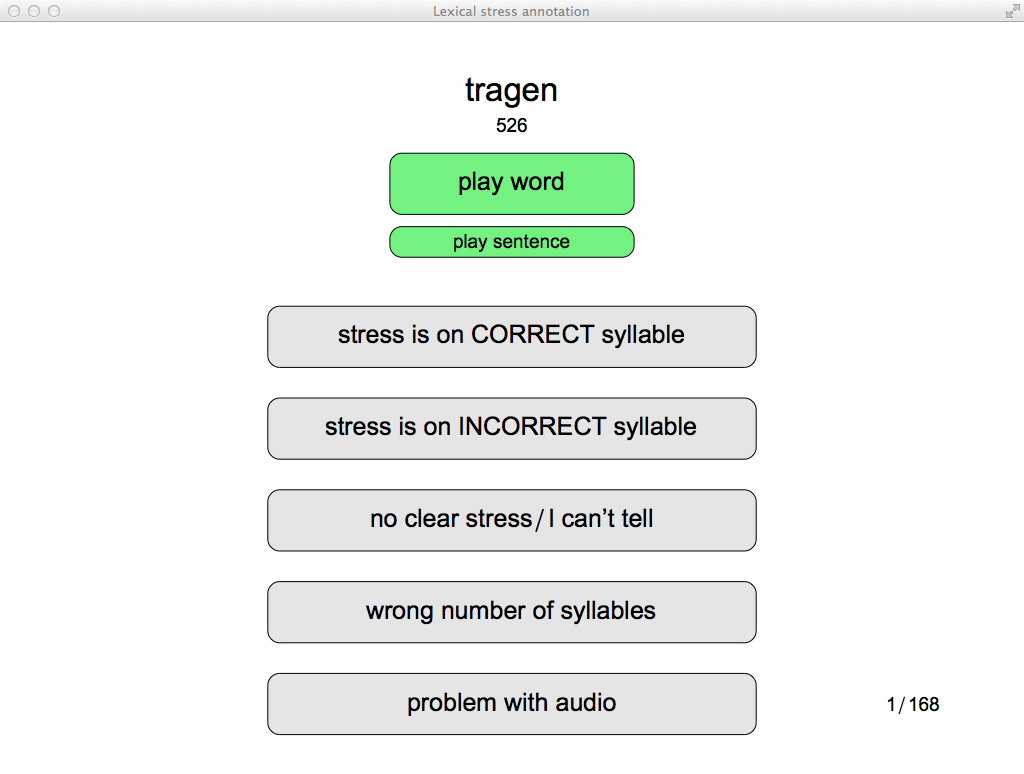
\includegraphics[width=\textwidth]{img/screenshots/AnnotationTool}
			\caption[A screenshot of the graphical annotation tool scripted in Praat.]{A screenshot of the graphical annotation tool scripted in Praat. Green buttons allow the annotator to listen to  the word and sentence utterances. Gray buttons allow the annotator to record their judgment of stress accuracy; from top to bottom, the buttons correspond to the labels [correct], [incorrect], [none], [bad\_nsylls], and [bad\_audio]. \TODO{border around graphic}}
			\label{fig:annotationtool}
		\end{figure}
		
		\TODO{some kind of section wrap-up?}
		
	
	\section{Inter-annotator agreement}
	\label{sec:lexstress:agreement}	
	
	To create a useful CAPT system for lexical stress errors in nonnative German, i.e. to automatically detect whether a student has made a lexical stress error in a given utterance, it is helpful to have an understanding of the difficulty of the error-detection task, not only for machines but for humans. It is therefore useful to analyze the collected stress accuracy judgments in terms of inter-annotator agreement, in order to gain insight into the nature of the challenge this task presents. If it is uncommon for human annotators to agree about whether a given lexical stress realization is correct or incorrect, this may indicate that  identifying lexical stress errors is a challenging task, and one which an automatic system should also be expected to have difficulty with. If, on the other hand, human annotators are generally in strong agreement, this may reflect a lower level of difficulty, and give reason to judge the performance of an automatic system by a higher standard.  
	
	As stated in the previous section,
	%\cref{sec:lexstress:data}, 
	lexical stress realizations in a total of 669 word utterances were each assigned to one of five classes by multiple annotators, based on whether the annotator judged the production to have correctly placed stress, incorrectly placed stress, no clear stress placement, or other problems which prevented the annotator from making a judgment about the lexical stress accuracy. The agreement between these judgments was calculated for each pair of annotators who overlapped, i.e. labeled any of the same tokens. 
	\TODO{matrix of pairwise tokens in common (or just x/o to show which annotators overlapped?}
	%This section describes how this agreement was calculated, and the following sections \cref{sec:agreement:overall, sec:agreement:native, sec:agreement:expertise} present an analysis of the resulting inter-annotator agreement statistics. Finally, 
		Two metrics were used to quantify agreement between a pair of annotators: the simple percentage of observed agreement, and Cohen's Kappa statistic ($\kappa$). 
		
		For a given pair of annotators, percentage agreement is calculated as the number of tokens to which both annotators assigned the same label, divided by the total number of tokens labeled by both annotators \TODO{as formula?}. Possible values for percentage agreement range from 0\%, representing complete disagreement between annotators, to 100\%, representing complete agreement. This simple metric ignores the probability of annotators agreeing by chance, and therefore may give a somewhat optimistic picture of inter-annotator agreement, but nevertheless serves as a basic, easy-to-interpret preliminary indication of the reliability of the collected judgments.
		
		To account for chance agreements not captured by the simple percentage of agreement, a second, more robust measure of inter-annotator agreement, Cohen's $\kappa$ \citep{Cohen1960}, was also calculated for each pair of annotators. For a given pair of annotators who have labeled the same tokens, $\kappa$ is computed as
		\[
		\kappa = \frac{p_a-p_c}{1-p_c}
		\]
		where $p_a$ is the proportion of tokens assigned the same label by both annotators (i.e. the simple percentage agreement just described) and $p_c$ is the proportion of tokens which can be expected to receive the same label from both annotators purely by chance. The latter thus represents the probability of the two annotators agreeing by chance, and is calculated for a pair of annotators $A$ and $B$ as
		\[
		p_c = \sum_{s \in S} p_A(s) \times p_B(s)
		\]
		where $s$ is one of the stress judgments in the set of possible labels $S$:
		\[S = \{\text{[correct]}, \text{[incorrect]}, \text{[none]}, \text{[bad\_nsylls]}, \text{[bad\_audio]}\}\]
		and $p_A(s)$ is the proportion of tokens assigned the label $s$ by annotator $A$, calculated as the number of tokens assigned label $s$ by annotator $A$ divided by the total number of tokens labeled by annotator $A$; $p_B(s)$ is calculated in the same way for annotator $B$.
		%and $p_A(s)$ and $p_B(s)$ are the proportion of tokens assigned the label $s$ by annotators $A$ and $B$, respectively. The value of $p_A(s)$ is calculated as the number of tokens assigned label $s$ by annotator $A$ divided by the total number of tokens labeled by annotator $A$. 
		As $\kappa$ thus accounts for the probability of two annotators assigning a token the same label purely by chance, it provides a more conservative representation of inter-annotator agreement. A $\kappa$ value of 0 indicates that the annotators do not agree any more than would be expected by chance. If agreement between annotators is less than chance, $\kappa$ will take a value below 0. The maximum possible value of $\kappa$ is 1.00, which indicates perfect agreement between annotators.
		
		In the following sections, both measures are provided in the hopes of presenting a more comprehensive picture of inter-annotator agreement than either metric can convey alone.  
		
		\TODO{Anything else to say here?}
		
		\subsection{Overall agreement}
		\label{sec:agreement:overall}
		
		
		To obtain an overall measure of inter-annotator agreement for this lexical stress assessment task, the agreement between each pair of overlapping annotators was quantified by the metrics discussed in the previous section, and the minimum, median, mean, and maximum values over all pairwise comparisons were computed; these values are given in \cref{tab:agreement:overall}.
	Though this provides a rather coarse-grained picture of the overall agreement, this simple analysis already points to a few interesting observations. First of all, we observe that the mean and median percentage agreement are near 55\%, indicating that, roughly speaking, annotators agree just slightly more often than they disagree; \TODO{\textit{fix:} this is not necessarily an encouraging ratio}. 
	%The $\kappa$ values are somewhat more difficult to interpret, but i
	Turning to the $\kappa$ values, if we consider that $\kappa = 0$ represents agreement purely by chance while $k = 1$ represents perfect, meaningful agreement, the fact that the mean and median $\kappa$ values between annotators are somewhere near 0.25 indicates that the agreement observed between annotators is closer to what would be expected simply by chance than to agreement that would indicate high reliability \TODO{\textit{remove?:} or some type of objective truth}. Looking next at the minimum and maximum values, we observe that while some pairs of annotators seem to exhibit relatively high agreement, 
	%removing this because it's not certain that these numbers correspond to the same pair:
	%with one pair reaching over 80\% agreement and a $\kappa$ over 0.6, 
	indicating \TODO{\textit{too fuzzy?} reasonably reliable} judgments, other pairs have very low agreement; in one case, with 23.21\% agreement, the annotators seem to be closer to perfect disagreement than perfect agreement, and the corresponding $\kappa$ being below zero indicates that they agreed even (slightly) less than one would expect if they were merely labeling utterances randomly. 

		\begin{table}[htb]
			\centering
			\caption{Overall pairwise agreement between annotators  \TODO{transpose this table so it's consistent with \cref{tab:agreement:L1} and \cref{tab:agreement:expertise}}}
			\begin{tabular}{lrrrr}
				\toprule
				Agreement measure &	Minimum	& Median &	 Maximum &	 Mean\\
				\midrule
				Percentage agreement &	23.21\%	& 55.36\%	& 83.93\%	& 54.92\% \\
				Cohen's $\kappa$ & 	-0.01	& 0.26	& 0.61	& 0.23 \\
				\bottomrule
			\end{tabular}
			\label{tab:agreement:overall}
		\end{table}
	
	\TODO{Is this section even meaningful? Should it be left out?} It seems, then, that there may be stark differences in reliability from annotator to annotator. Analysis of the set of pairwise comparisons between a given annotator and all overlapping annotators provides more insight into that annotator's individual reliability; \cref{fig:agreement:annotators} illustrates the pairwise agreements involving each of the 15 annotators. These figures should be interpreted with caution because they do not account for differences in the number of overlapping annotators/tokens available for each annotator \TODO{reference overlap table}; nonetheless, it seems that there is indeed some noticeable variation from annotator to annotator \TODO{finish this paragraph}
		\TODO{table of percent/kappa min/avg/max by annotator, since graphs are difficult to read precisely?}
		
		\begin{figure}[htb]
			\centering
			
			\begin{subfigure}[b]{\textwidth}
				\centering
				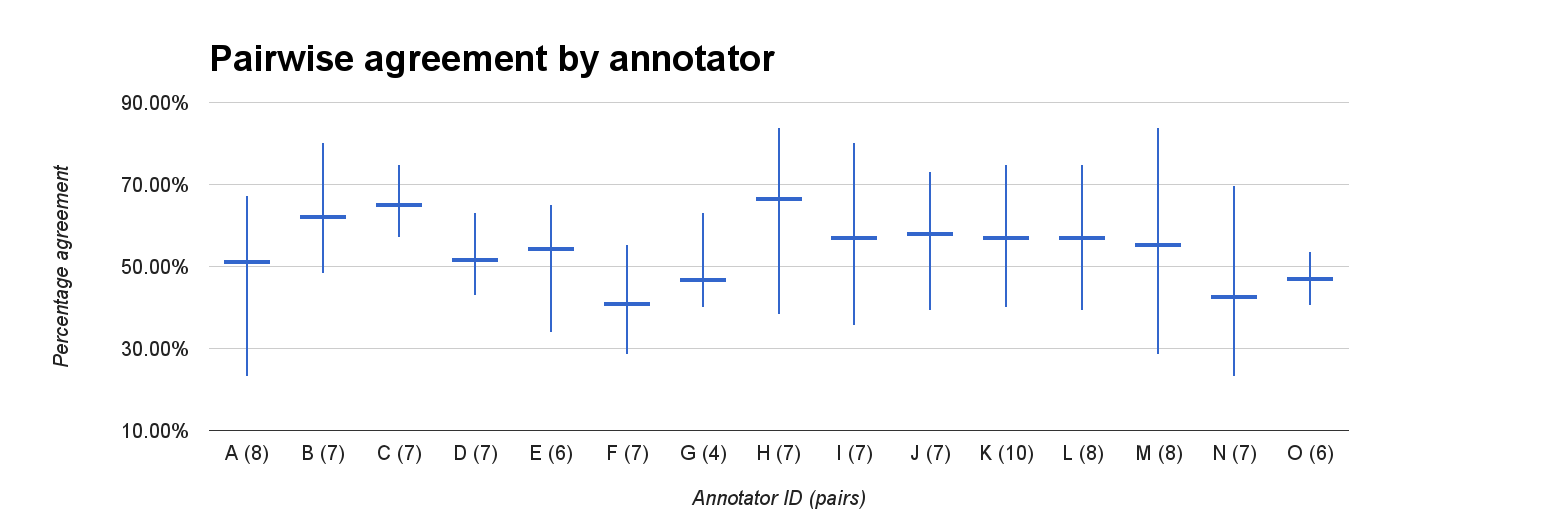
\includegraphics[width=\textwidth]{img/annotation/pairAgreeAnnotators}
				\caption{Percent agreement}
				\label{fig:agreement:annotators:pct}
			\end{subfigure}%
			
			\begin{subfigure}[b]{\textwidth}
				\centering
				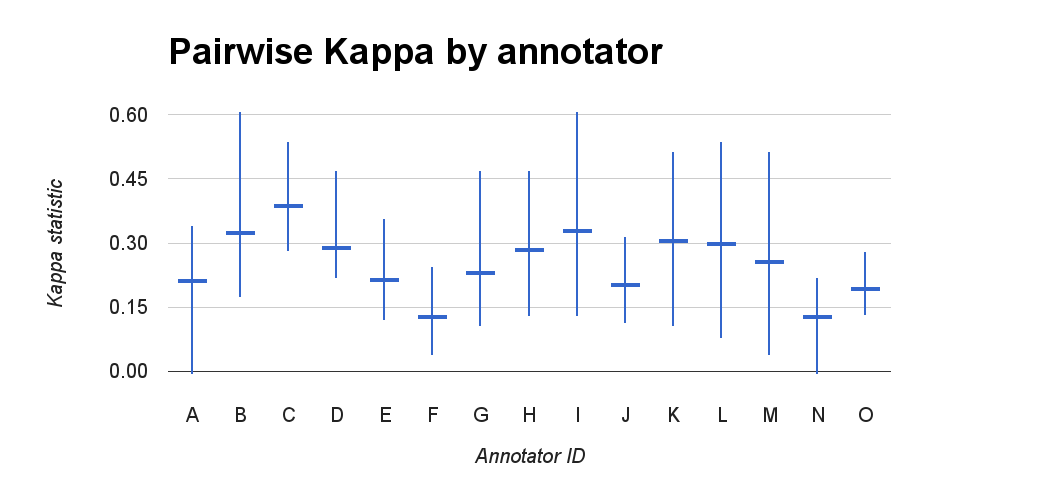
\includegraphics[width=\textwidth]{img/annotation/pairKappaAnnotators}
				\caption{Cohen's Kappa statistic}
				\label{fig:agreement:annotators:k}
			\end{subfigure}%
			
			\caption[Pairwise agreement statistics by annotator]{Each annotator's pairwise agreement with all other annotators with whom they overlapped. Numbers in parentheses indicate the number of pairwise comparisons involving each annotator. The bottom of each vertical bar represents the minimum pairwise value, the top the maximum. Horizontal bars indicate mean pairwise values.}
			\label{fig:agreement:annotators}
		\end{figure}
		
		It is also of interest to analyze the overall inter-annotator agreement for each word type in the annotated sub-corpus. As \cref{fig:agreement:words} illustrates, there are noticeable differences between word types, with annotators exhibiting relatively high agreement on certain words (e.g. \textit{E-mail}, \textit{halten}, and \textit{Pollen}), and on other words (e.g. \textit{manche} and \textit{Ringen}) exhibiting agreement values closer to chance. \TODO{DISCUSSION (reference error breakdown by word in sec:results:overall}
		
		
		\begin{figure}[htb]
			\centering
			
			\begin{subfigure}[b]{\textwidth}
				\centering
				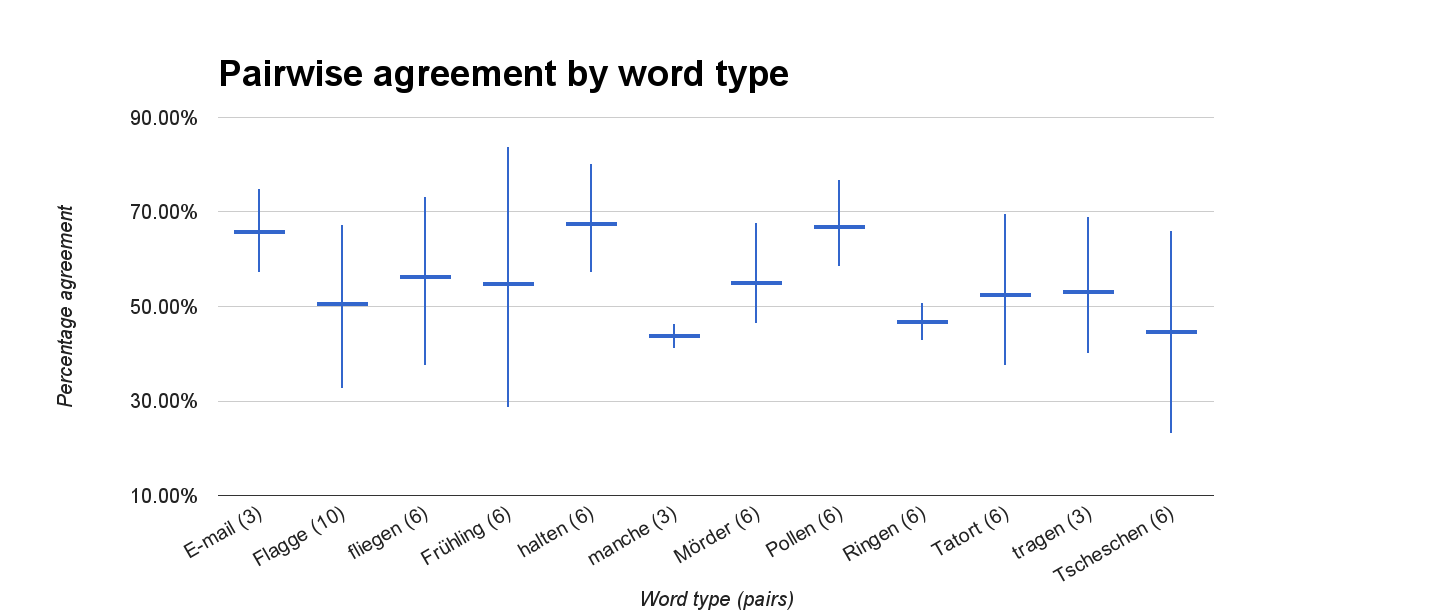
\includegraphics[width=\textwidth]{img/annotation/pairAgreeWords}
				\caption{Percent agreement}
				\label{fig:agreement:words:pct}
			\end{subfigure}%
			
			\begin{subfigure}[b]{\textwidth}
				\centering
				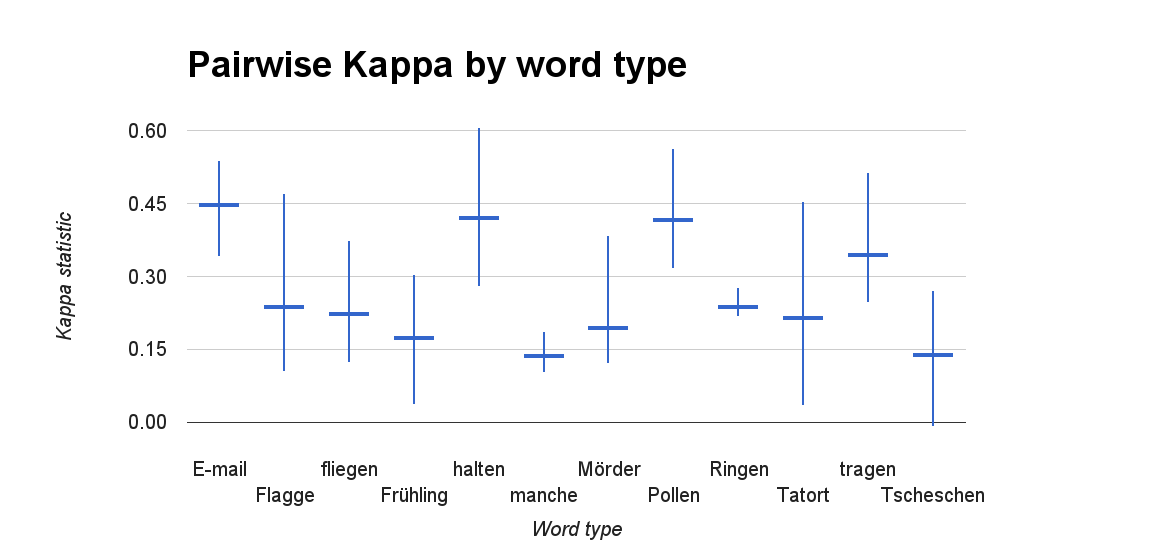
\includegraphics[width=\textwidth]{img/annotation/pairKappaWords}
				\caption{Cohen's Kappa statistic}
				\label{fig:agreement:words:k}
			\end{subfigure}%
			
			\caption[Pairwise agreement statistics by word type]{Pairwise agreement between annotators for each word type. Numbers in parentheses indicate the number of pairwise comparisons available for each word type. The bottom of each vertical bar represents the minimum pairwise value, the top the maximum. Horizontal bars indicate average pairwise values.}
			\label{fig:agreement:words}
		\end{figure}
		
		
	
		
		\TODO{Move this?} On the whole, then, it seems that inter-annotator agreement in this lexical stress error annotation task is relatively low, which indicates that the task of assessing a given lexical stress realization as correct or incorrect is a relatively difficult one. 
	
		\TODO{transition}
	
		%\subsubsection{Native vs. nonnative annotators}
		\subsection{Native vs. nonnative annotators}
		\label{sec:agreement:native}

		
		
		Going beyond the coarse-grained analysis of inter-annotator agreement described in the previous section, we come now to the second question raised at the beginning of this chapter:
		
		\textit{Are there differences in how native and non-native German speakers identify errors?}
		
		\TODO{expectations/speculations of what we will find?}
		
		To answer this question, it is useful to look at the inter-annotator agreement between native and non-native annotators, as well as at the distribution of label types within each group. 
		
		\Cref{fig:agreement:L1} illustrates the inter-annotator agreement for all pairs in which one annotator was a native German speaker and the other a non-native speaker, as well as agreement between pairs in which both annotators were native speakers. Due to the small size of the non-native group (3 annotators) and the aforementioned technical problems with annotator G's data (see \cref{sec:lexstress:annotators}), there was very little overlap between non-native annotators (only one pairwise comparison), preventing meaningful analysis of agreement within the non-native group. The precise mean, maximum, median, and minimum pairwise values for the two agreement metrics are listed in \cref{tab:agreement:L1}, for both  native-nonnative pairs and native-native pairs. 
		
		Looking at these statistics, we see little difference between the two types of pairs; in particular, the mean percentage agreement and $\kappa$ values for native-nonnative and native-native pairs are quite close. If anything, it would appear that agreement within the native annotator group is slightly lower and more varied than agreement between the native and nonnative groups, though this may be explained by the larger number of native-native pairs compared to native-nonnative. It would therefore seem that these inter-annotator statistics do not tell us much about difference between how the two groups of annotators judge lexical stress accuracy.
		
		
		\begin{table}[htb]
			\centering
			\caption{Inter-annotator agreement between native and non-native annotators (pairwise)}
			%\begin{tabularr}{\textwidth}{lXXXX}
			\begin{tabular}{lrrrr}
			\toprule
			& \multicolumn{2}{c}{Native vs. nonnative} & \multicolumn{2}{c}{Native vs. native} \\
			\cmidrule(lr){2-3} \cmidrule(lr){4-5}
			& \% Agreement & Cohen's $\kappa$ & \% Agreement & Cohen's $\kappa$  \\
			\midrule
Mean	&56.98\%	 & 0.29  & 53.87\%	& 0.25\\
Maximum&	76.79\%	& 0.56 & 83.93\%	 & 0.61\\
Median	& 57.14\%	 &0.25 &  50.91\%	& 0.23 \\
Minimum	&32.65\%	 & 0.10 &  23.21\% &	-0.01\\
			\bottomrule
			\end{tabular}
			\label{tab:agreement:L1}
		\end{table} 
		
		\begin{figure}[htb]
			\centering
			
			\begin{subfigure}[b]{.5\textwidth}
				\centering
				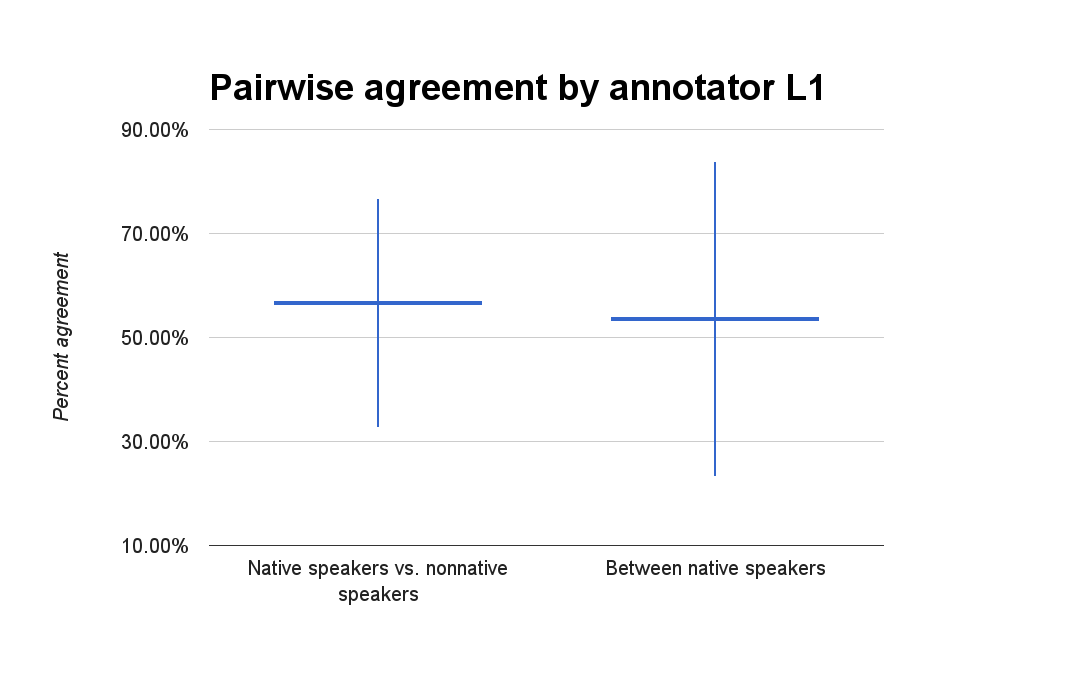
\includegraphics[width=\textwidth]{img/annotation/pairAgreeL1}
				\caption{Percent agreement}
				\label{fig:agreement:L1:pct}
			\end{subfigure}%
			~
			\begin{subfigure}[b]{.5\textwidth}
				\centering
				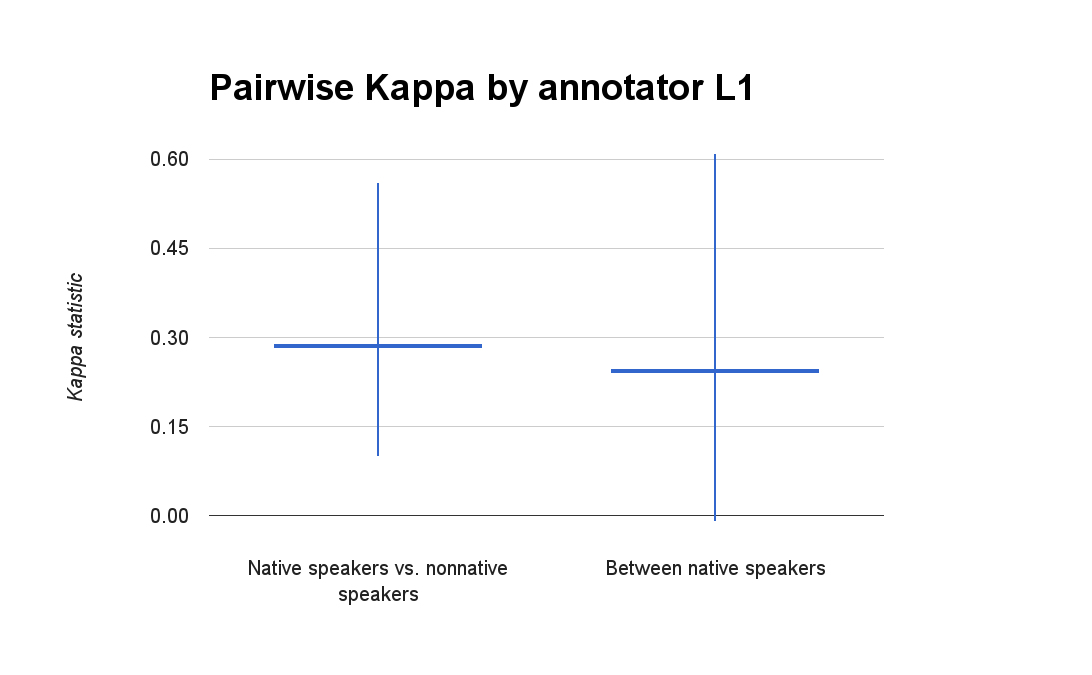
\includegraphics[width=\textwidth]{img/annotation/pairKappaL1}
				\caption{Cohen's Kappa statistic}
				\label{fig:agreement:L1:k}
			\end{subfigure}%
			
			\caption[Pairwise agreement statistics by annotator L1 group]{Pairwise agreement between annotators based on their L1  (native or nonnative German speaker). The bottom of each vertical bar represents the minimum pairwise value, the top the maximum. Horizontal bars indicate average pairwise values.}
			\label{fig:agreement:L1}
		\end{figure}
		
		

		However, in comparing the relative frequencies of the different labels assigned by annotators in these two L1 groups, a more noticeable difference between the groups begin to emerge. As illustrated in \cref{fig:l1pies}, we observe that the native and nonnative speakers judge utterances as having correct lexical stress with approximately the same frequency: 52.7\% of native annotators' judgments are \textbf{[correct]}, vs. 57.3\% for nonnative annotators. However, nonnative speakers seem to choose the \textbf{[none]}
		%``no clear stress/I can't tell'' 
		label somewhat more frequently than native speakers (21.3\% vs. 11\%); this could indicate that nonnative speakers are less confident about how stress should be realized in German, resulting in less certainty about whether a given utterance is correct or not. \TODO{update/verify this paragraph}
		
		
			\begin{figure}[htb]
				\centering
				\begin{subfigure}[b]{.5\textwidth}
					\centering
					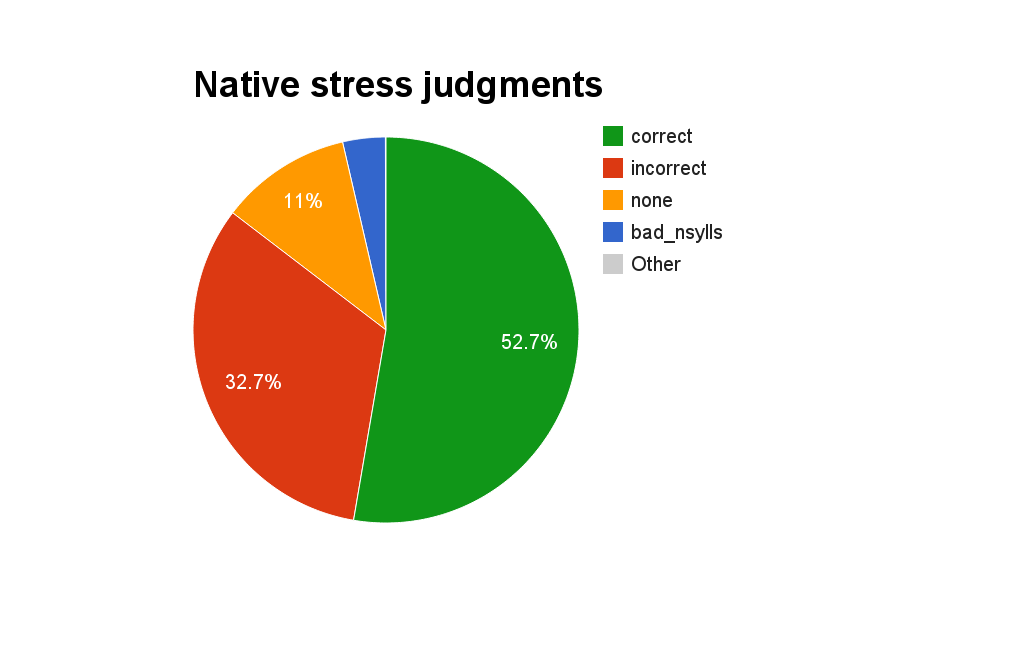
\includegraphics[width=\textwidth]{img/annotation/nativePie}
					\caption{Native annotators}
					\label{fig:l1pies:native}
				\end{subfigure}%
				~
				\begin{subfigure}[b]{.5\textwidth}
					\centering
					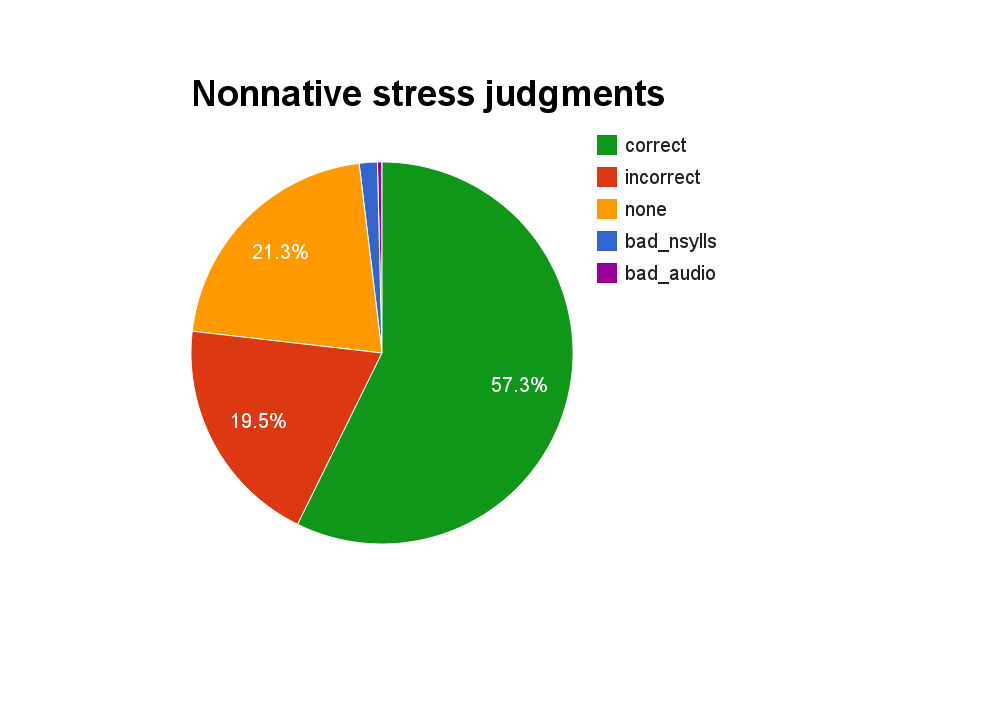
\includegraphics[width=\textwidth]{img/annotation/nonnativePie}
					\caption{Nonnative annotators}
					\label{fig:l1pies:nonnative}
				\end{subfigure}%
				\caption{Stress judgments made by native and nonnative German speakers}
				\label{fig:l1pies}
			\end{figure}
			
		Though the differences between native and nonnative annotators are interesting \TODO{from the perspective of X}, the ultimate goal of this thesis project is to create a CAPT tool which will help L1 French speakers be more intelligible when speaking German as L2, and therefore the way in which native German speakers perceive lexical stress in non-native speech is of more relevance to this work than the way it is perceived by non-native speakers. Therefore, the remainder of this chapter is concerned exclusively with the judgments of native annotators, and judgments by non-native annotators are not included in the analyses that follow.
			
		
		\subsection{Expert vs. novice annotators}
		\label{sec:agreement:expert}
		
		
		
	\TODO{Transition} This section seeks to answer the last of the questions raised at the beginning of the chapter concerning inter-annotator agreement in the stress-annotated IFCASL sub-corpus, namely:
	
	\textit{Are there differences in how expert and novice annotators identify lexical stress errors?}
	
	Given the general difficulty of the task of identifying lexical stress errors, evidenced by relatively low overall inter-annotator agreement as discussed in \cref{sec:agreement:overall} above, it might seem reasonable to suppose that training in phonetics/phonology or experience annotating (non-native) speech might have a positive impact on an annotator's ability to reliably judge the accuracy of lexical stress realizations by non-native speakers. However, it once again bears mentioning that the ultimate goal of this work is to help L2 learners communicate intelligibly in German, and it can safely be assumed that in the vast majority of cases such learners will be communicating more often with native speakers who possess little formal knowledge of speech science than with expert phoneticians. Therefore, even if differences in reliability do exist between expert and novice annotators, it is important that the perception of non-native lexical stress errors by non-experts not be ignored in favor of perception of such errors by experts \TODO{reword that, or just scrap this sentence?}. 
	
	%\TODO{mention that we're trying to train nonnative speakers to communicate in the L2, which means their speech will be ``evaluated'' by novices (native speakers), so we don't want to limit ourselves to expert judgments}

	\TODO{Better transition needed here?}
	
	Just as the previous section analyzed native vs. non-native annotations in terms of inter-annotator agreement and differences in label distributions between those groups, this section uses analogous data to investigate the differences between annotators of the three different expertise levels -- expert (exp.), intermediate (int.), and novice (nov.) -- described in \cref{sec:lexstress:annotators} above.
	
	To determine inter-annotator agreement between the three expertise groups, percentage agreement and $\kappa$ were tabulated for each pairing of annotators from different groups, i.e. for each of the following three pair types:
	
	\begin{itemize}
	\item{Expert annotator vs. novice annotator}
	\item{Expert annotator vs. intermediate annotator}
	\item{Novice annotator vs. intermediate annotator}
	\end{itemize}
	
	Additionally, pairwise agreement was tallied for pairings between two intermediate annotators, as a measure of inter-annotator agreement within this expertise group. Due to the small size of the expert and novice groups (two and three annotators, respectively), as well as the fact that expert annotators were deliberately not assigned overlapping tokens to label in an effort to maximize the number of tokens labeled by at least one expert \TODO{does that contradict the above statement about novice judgments being just as important as expert ones?}, overlap within these groups was insufficient to calculate meaningful intra-group agreement statistics, so none are reported here. The small size of these two groups should also be kept in mind throughout the following analysis, as we should hesitate to draw firm conclusions from such small samples. 
		
		The agreement measures between groups and within the intermediate group are presented in \cref{tab:agreement:expertise} and illustrated in \cref{fig:agreement:expertise}. As these figures show, the mean values of both percentage agreement and $\kappa$ between the different expertise groups are quite close, and close to the overall means for all annotator pairs;  interestingly, the highest mean percentage agreement observed in this comparison (though only by a small margin) is that of expert-novice pairings, which might be a preliminary indication that there is no relevant difference in reliability between expertise levels. 
			
		
		
		\begin{table}[htb]
			\centering
			\caption{Pairwise agreement between expertise groups \TODO{explain abbreviations}}
			\begin{tabularx}{\textwidth}{lXXXXXXXX}
				\toprule
		& \multicolumn{2}{c}{Exp vs. Nov} & \multicolumn{2}{c}{Exp vs. Int} & \multicolumn{2}{c}{Nov vs. Int} & \multicolumn{2}{c}{Int vs. Int} \\
	&\% Agr.	& $\kappa$	&\% agr. &	$\kappa$&	\% agr.	& $\kappa$	&\% agr. & $\kappa$ \\
	\midrule
Mean	& 57.89\%	& 0.23	& 55.30\%	& 0.23	& 52.12\%	& 0.26	& 51.44\%	& 0.23 \\
Maximum	& 71.43\%	& 0.44	& 83.93\%	& 0.32	& 71.43\% & 	0.47	& 80.36\%	& 0.61 \\
Median	& 68.46\%	& 0.24	& 49.95\%	& 0.25	& 51.70\%	& 0.26	& 47.58\%	& 0.22\\
Minimum	& 23.21\%	& -0.01	& 33.93\%	& 0.10	& 35.71\%	& 0.08	& 28.57\%	&  0.04 \\
				\bottomrule
			\end{tabularx}
			\label{tab:agreement:expertise}
		\end{table}
			
		
		
		\begin{figure}[htb]
			\centering
			
			\begin{subfigure}[b]{.5\textwidth}
				\centering
				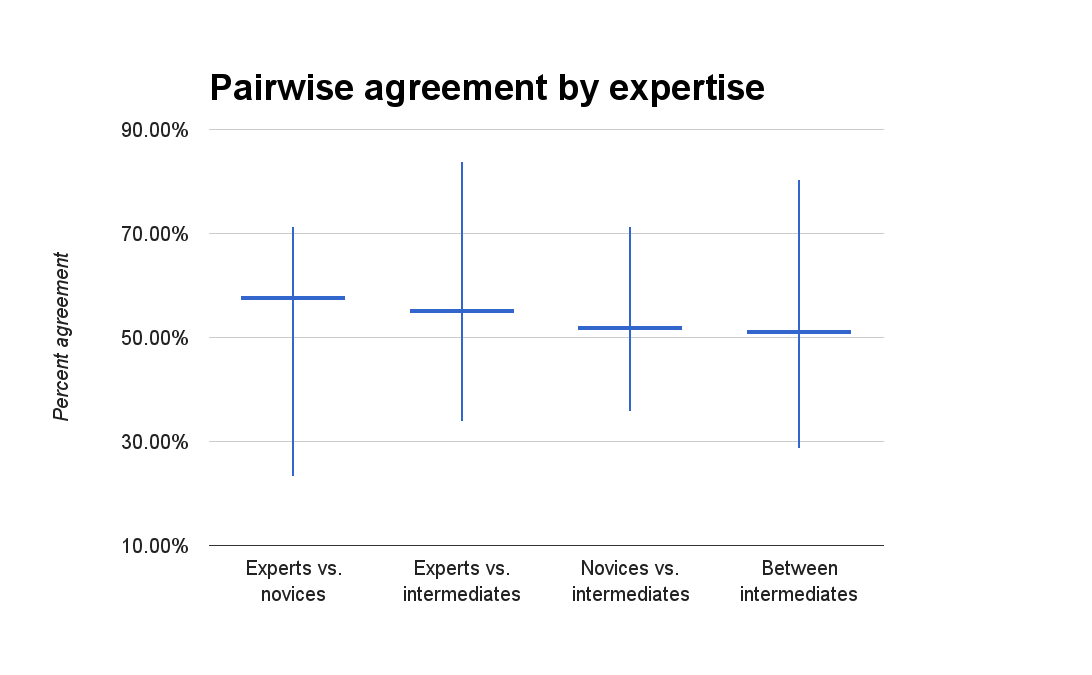
\includegraphics[width=\textwidth]{img/annotation/pairAgreeExpertise}
				\caption{Percent agreement}
				\label{fig:agreement:expertise:pct}
			\end{subfigure}%
			~
			\begin{subfigure}[b]{.5\textwidth}
				\centering
				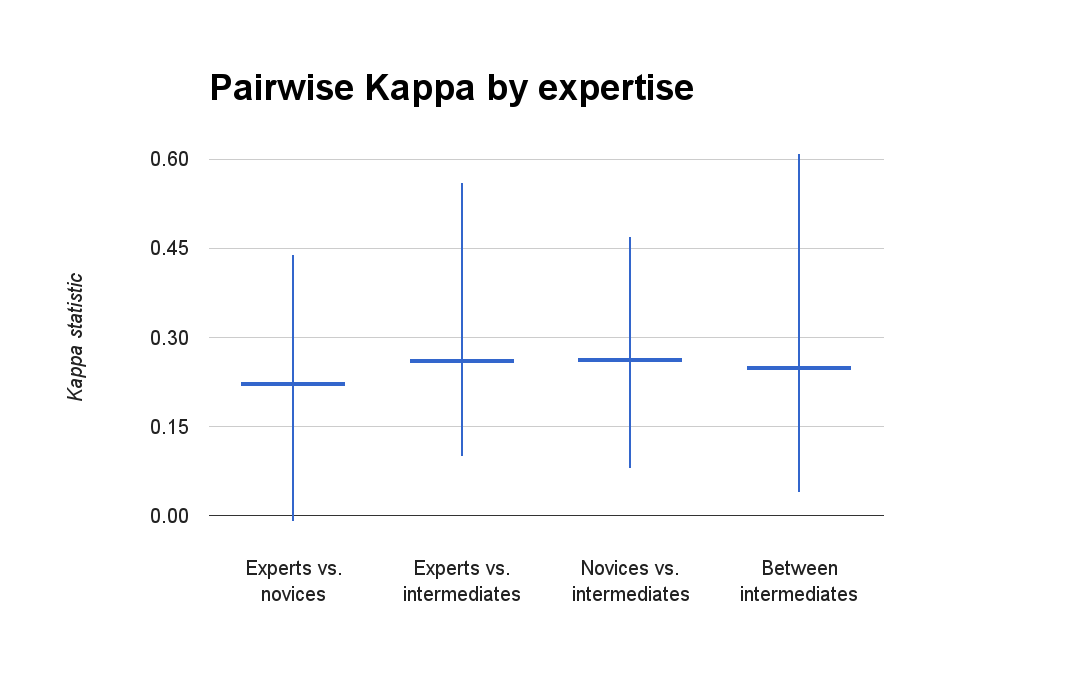
\includegraphics[width=\textwidth]{img/annotation/pairKappaExpertise}
				\caption{Cohen's Kappa statistic}
				\label{fig:agreement:expertise:k}
			\end{subfigure}%
			
			\caption[Pairwise agreement statistics by annotator expertise]{Pairwise agreement between annotators based on their level of expertise (expert, intermediate, or novice). The bottom of each vertical bar represents the minimum pairwise value, the top the maximum. Horizontal bars indicate average pairwise values.}
			\label{fig:agreement:expertise}
		\end{figure}
		
			\Cref{fig:expertisepies} illustrates the relative number of each label type as assigned by annotators of the three expertise levels described in \cref{sec:lexstress:annotators} above, and while any analysis of this data should bear in mind the small sample sizes of the expert and novice groups (two and three annotators, respectively), it does appear that some interesting differences may exist between the three groups. 
			
			Expert annotators seem to be far more ``generous'' in their labeling than intermediate or novice annotators, in that the experts assigned the \textbf{[correct]} label 73.6\% of the time, in contrast with 49.3\% and 54.8\% for the other two groups respectively. \TODO{\textit{person?:} One could} speculate that experts' familiarity with nonnative speech and knowledge of possible inter-speaker variations in lexical stress realization may be the cause for this willingness to ``accept'' a high proportion of utterances as correct. \TODO{too many scare quotes in this paragraph?}
			
			Another interesting difference can be observed between the intermediate and novice annotator groups: compared with the intermediate annotators, novices assign the \textbf{[none]} label less frequently (5.8\% of the time, versus 16.3\% for intermediates) and the \textbf{[bad\_nsylls]} label more frequently (8.4\% of the time, versus 2.1\% for intermediates). Still keeping in mind the discrepancy in sample sizes when comparing 10 intermediate annotators to three novices, \TODO{\textit{person?:} we might} speculate that if experts' extensive experience with nonnative speech could be an explanation for their ``generosity'' with the correct label, novice annotators' lack of experience with nonnative speech could in a similar way make them ``harsher'' in judging nonnative utterances as having an incorrect number of syllables. \TODO{This paragraph sucks. Also too many scare quotes.}
			
			%TODO include?
%			\begin{figure}[htb]
%				\centering
%				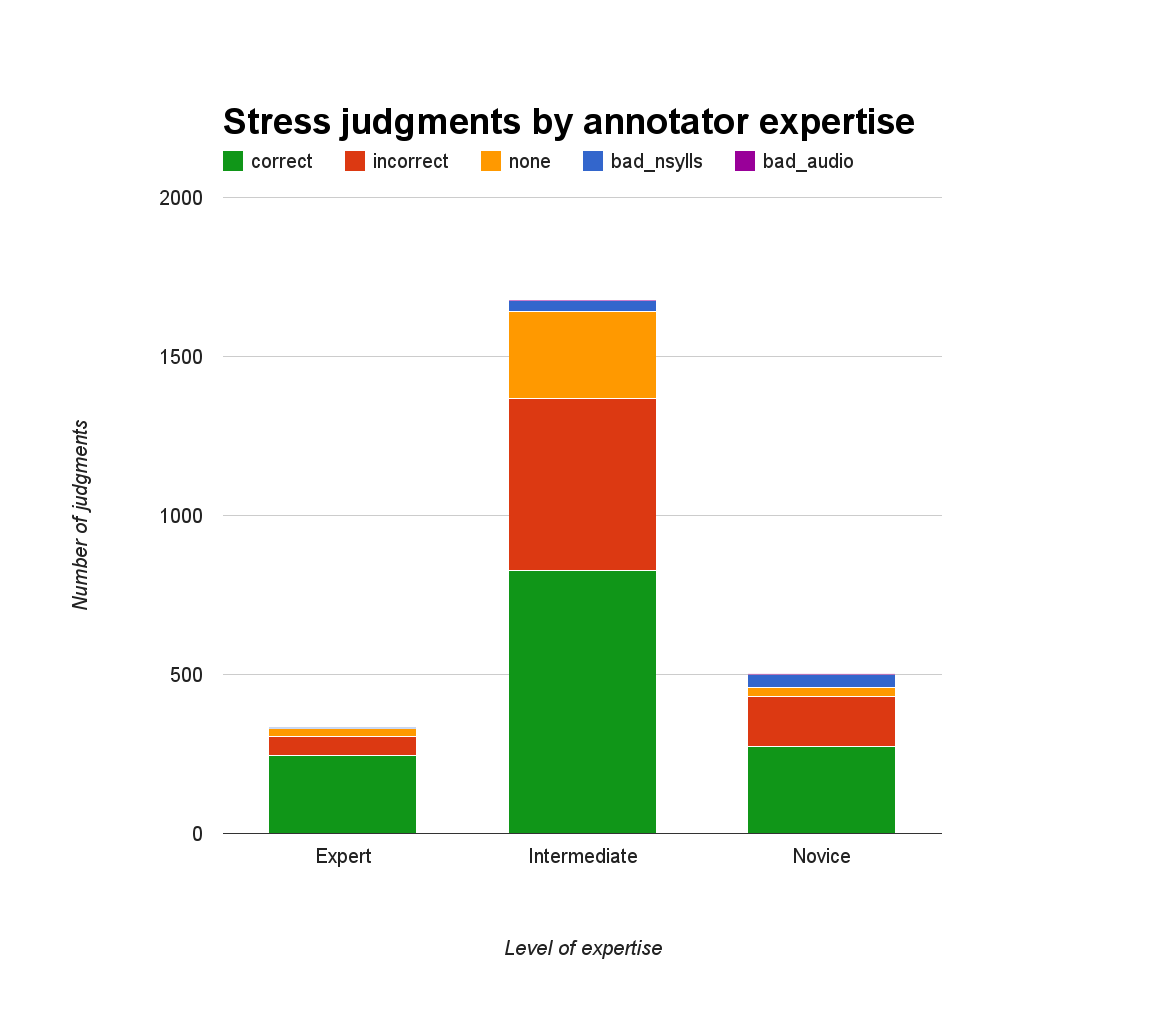
\includegraphics[width=\textwidth]{img/annotation/expertiseBars}
%				\caption{Stress judgments by annotator expertise}
%				\label{fig:expertisebars}
%			\end{figure}
			
			
			\begin{figure}[htb]
				\centering
				\begin{subfigure}[b]{.5\textwidth}
					\centering
					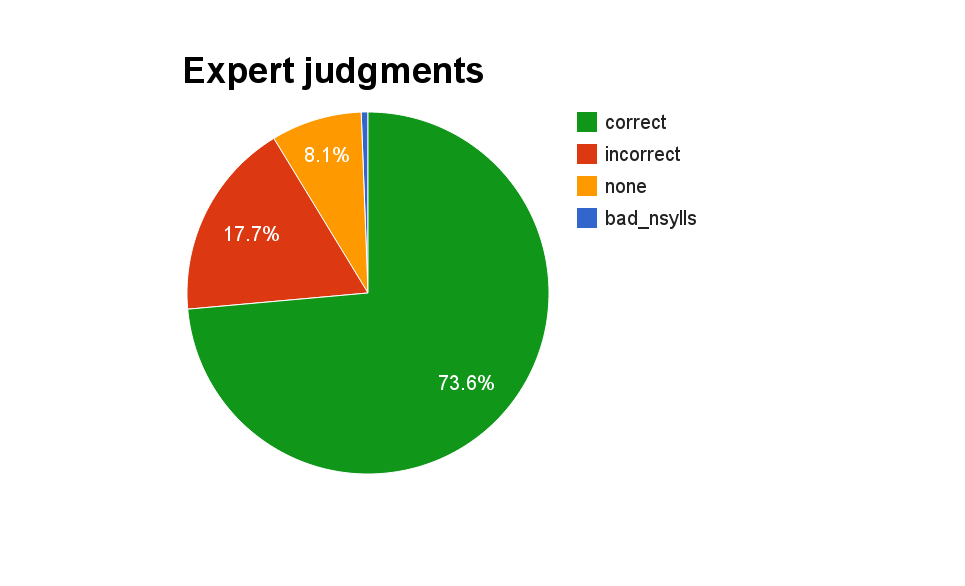
\includegraphics[width=\textwidth]{img/annotation/expertPie}
					\caption{Expert}
					\label{fig:expertisepies:expert}
				\end{subfigure}%
				
				\begin{subfigure}[b]{.5\textwidth}
					\centering
					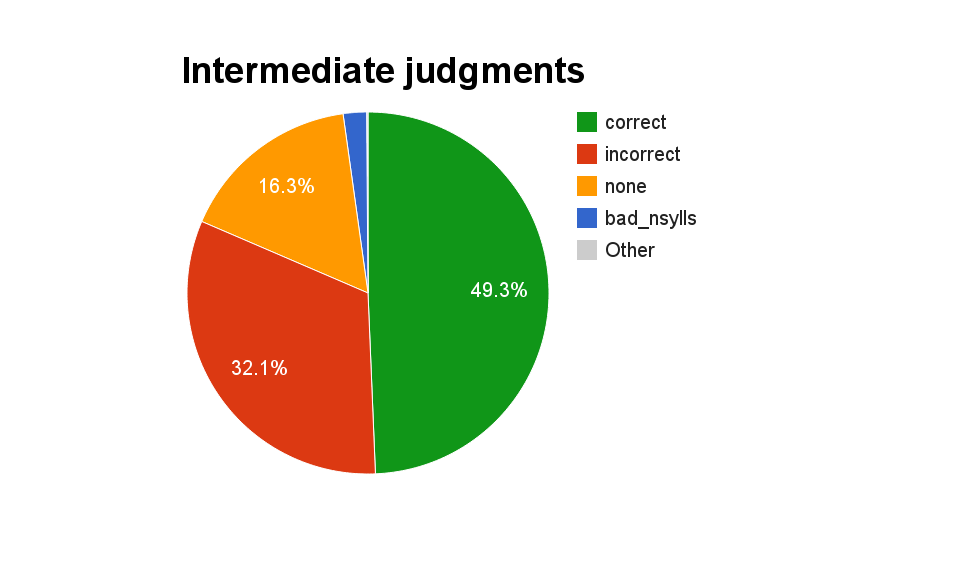
\includegraphics[width=\textwidth]{img/annotation/intermediatePie}
					\caption{Intermediate}
					\label{fig:expertisepies:intermediate}
				\end{subfigure}%
				~
				\begin{subfigure}[b]{.5\textwidth}
					\centering
					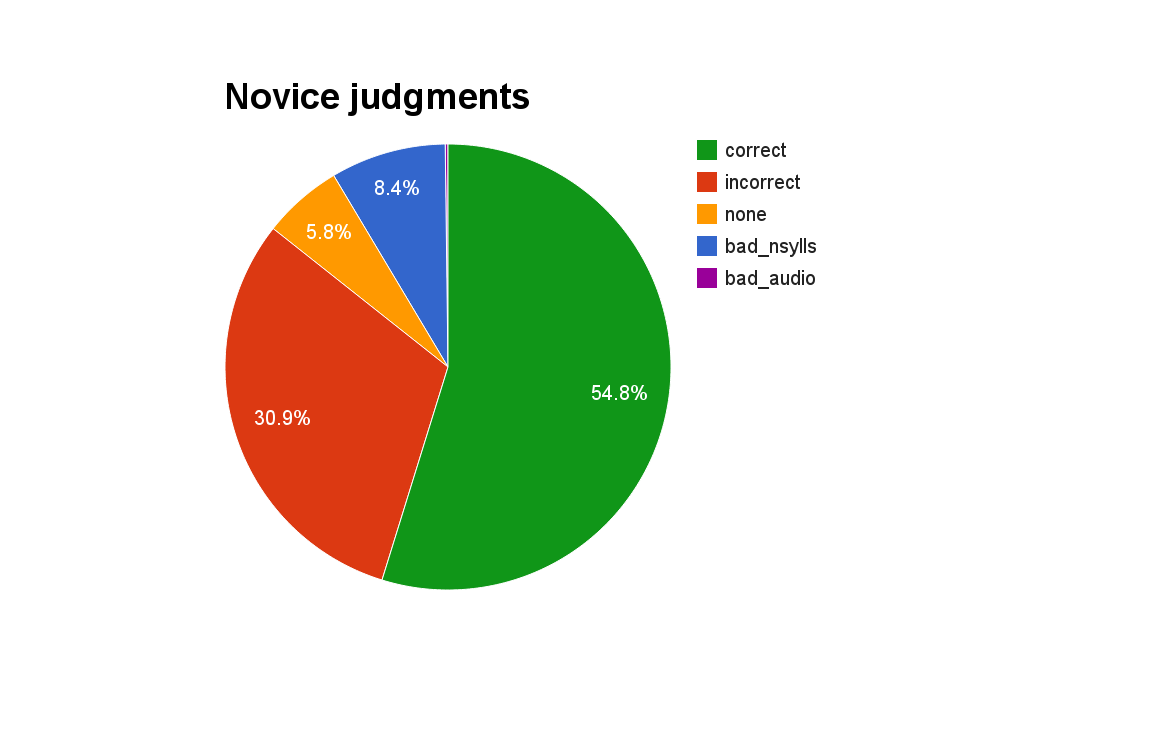
\includegraphics[width=\textwidth]{img/annotation/novicePie}
					\caption{Novice}
					\label{fig:expertisepies:novice}
				\end{subfigure}%
				\caption{Stress judgments by annotator expertise}
				\label{fig:expertisepies}
			\end{figure}
			
			
			\TODO{Conclusion}
			
		\subsection{Choosing gold-standard labels}
		\label{sec:agreement:gold}
		
		\TODO{Rephrase gold-standard  as ground truth or some other term?}
		
		As the previous sections have illustrated, having multiple annotators judge the accuracy of each lexical stress production was useful insofar as it led to some interesting observations about the difficulty of reliably assessing lexical stress accuracy and differences in how judgments by annotators with different native languages and levels of expertise compare. However, if the annotations are to be used for \TODO{training an automated error-diagnosis system}, each token in the sub-corpus must ultimately be assigned a single ``gold-standard'' label from the set of possibilities described in \cref{sec:lexstress:annotation} (\textbf{[correct]},\textbf{[incorrect]},\textbf{[none]},\textbf{[bad\_nyslls]},\textbf{[bad\_audio]}). 
		
		For 268 of the 669 tokens annotated, there was no disagreement whatsoever between annotators: for each of these 268 tokens, all annotators who labeled the token made the same judgment \TODO{How does this fit in with \cref{sec:agreement:overall}? Should it be mentioned there?}, making it easy to assign this label as the gold standard for this utterance. For another 265 tokens, a majority of annotators assigned the same label, though one or more annotators dissented, so assigning the majority-vote label as the gold standard is logical. Therefore, for a total of 533 tokens (approximately 80\% of the word utterances in the sub-corpus), the gold standard label was uncontroversial.
		
		However, choosing gold-standard labels for the remaining 116 utterances was a less straightforward task. 
		
				\TODO{Explain how a final label was decided for each token}

		Original rules:
		\begin{itemize}
		\item{if there is only one label or a majority vote, use that}
		\item{if one of the annotators is an expert (FZ, JJ, or RM), use that}
		\item{if [bad\_nsylls] is one of the best labels, ignore it}
		\item{if it was judged both correct and incorrect (i.e. both [correct] and [incorrect] are in the best labels), choose [none]}
		\item{if there are two best labels and one is [none], choose the more certain label (i.e. ignore [none])}
		\end{itemize}
		
		\begin{tabular}{ll}
				Original breakdown:\\
		ignore\_none &	 19 \\
ignore\_badsylls &	 0\\
no\_decision &	 0\\
incorrect+correct=none &	 36\\
single\_label &	 268\\
majority\_vote (533 - 268) &	 265\\
expert\_wins &	 81\\
		\end{tabular}
		

		New rules:
		\begin{itemize}
		
		\item{if there is only one label or a majority vote, use that}
		\item{if one of the annotators is an expert (FZ or JJ), use that}
		\item{if [bad\_nsylls] is one of the best labels, ignore it}
		%\item{\textit{the rest of these are \TODO{}}}
		\item{Be generous? (if anyone labeled it [correct], go with that)}
		\item{ignore [none]}
		%\item{...}
		\end{itemize}
		
		
		\begin{tabular}{ll}
		New breakdown:\\
		generosity &	 51 \\
no\_decision &	 0 \\ 
single\_label &	 268 \\ 
majority\_vote\_or\_single (subtract single from this) &	 533 \\
expert\_wins &	 68 \\ 
ignore\_badsylls &	 0 \\
ignore\_none &	 17 \\
		\end{tabular}
			

	\section{Results}
	\label{sec:lexstress:results}		
	
		\TODO{intro}		
			
			
			
		\subsection{Overall frequency of lexical stress errors}
		\label{sec:results:overall}
		
		\TODO{Maybe this section should go last instead of first?}
		
		%\subsubsection{Accuracy by L2 skill level}
		\subsection{Errors by L2 skill level}
		\label{sec:results:level}
		
			\TODO{text}
			
			%TODO exclude?
			\begin{figure}[htb]
				\centering
				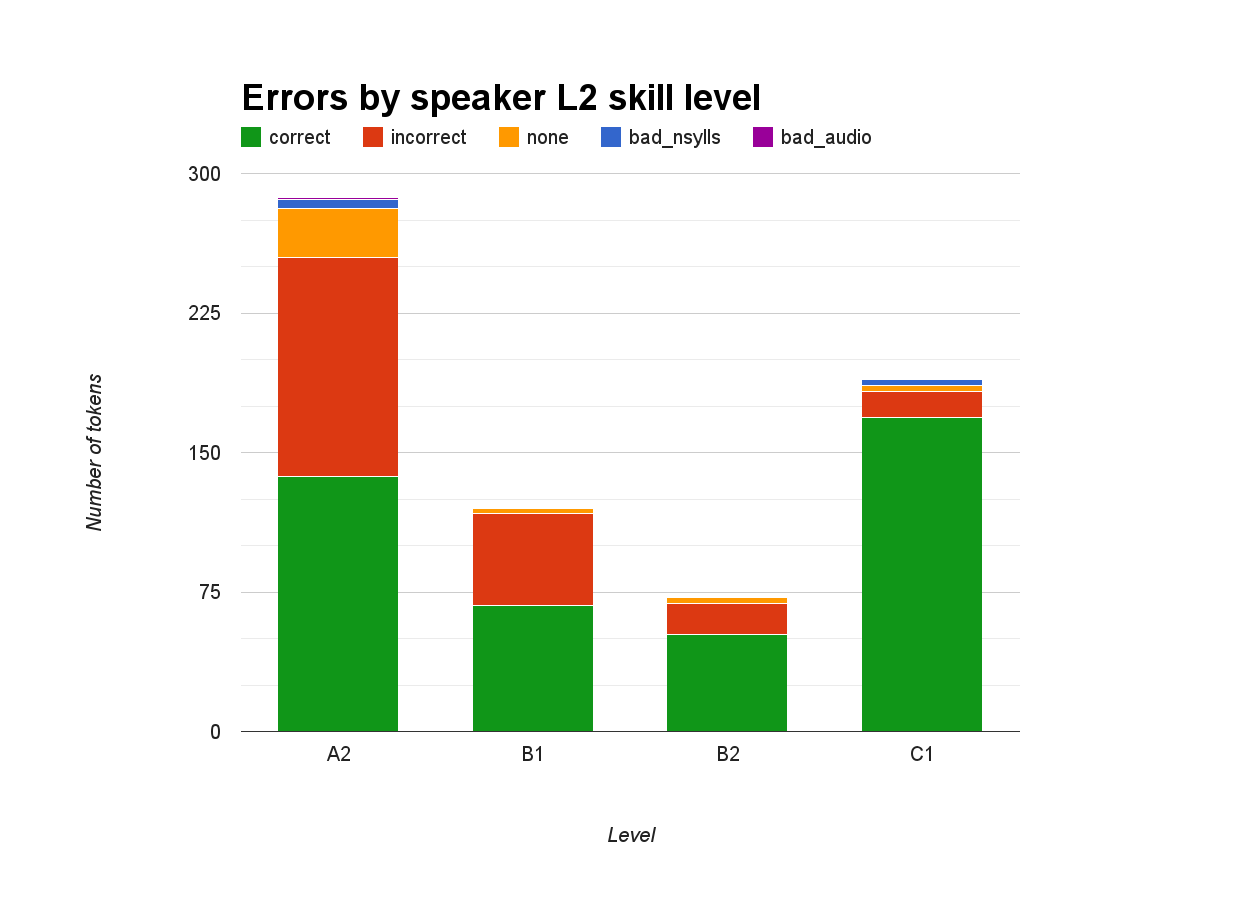
\includegraphics[width=\textwidth]{img/annotation/skillLevelBars}
				\caption{Stress judgments by speaker skill level \TODO{Exclude?}}
				\label{fig:levelbars}
			\end{figure}
		
		
			\begin{figure}[htb]
				\centering
				\begin{subfigure}[t]{0.5\textwidth}
					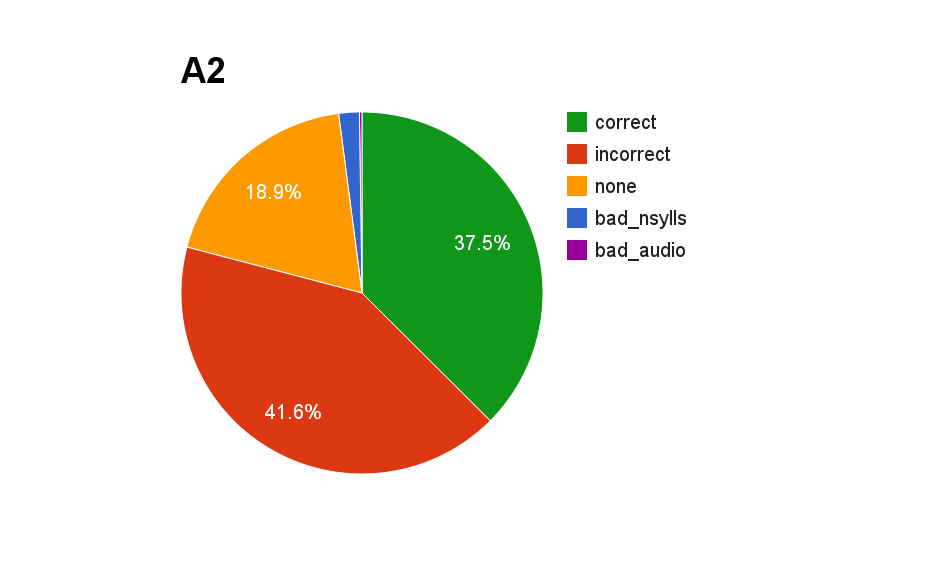
\includegraphics[width=\textwidth]{img/annotation/A2}
					\caption{A2}
					\label{fig:levelpies:A2}
				\end{subfigure}%
				~
				\begin{subfigure}[t]{0.5\textwidth}
					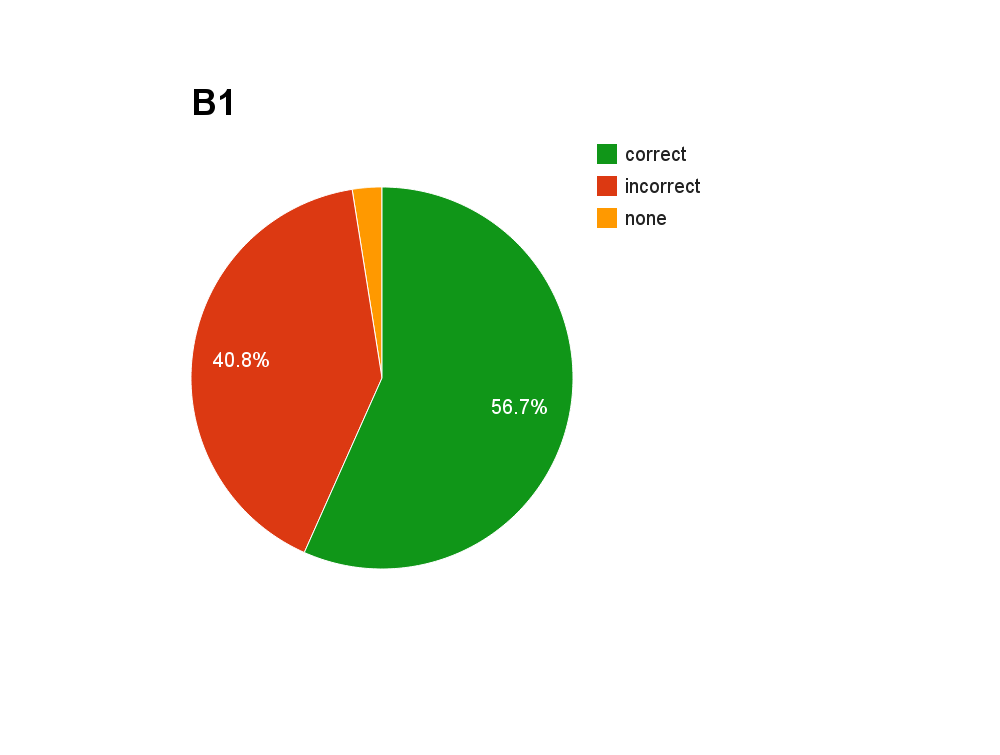
\includegraphics[width=\textwidth]{img/annotation/B1}
					\caption{B1}
					\label{fig:levelpies:B1}
				\end{subfigure}%
				
				\begin{subfigure}[b]{0.5\textwidth}
					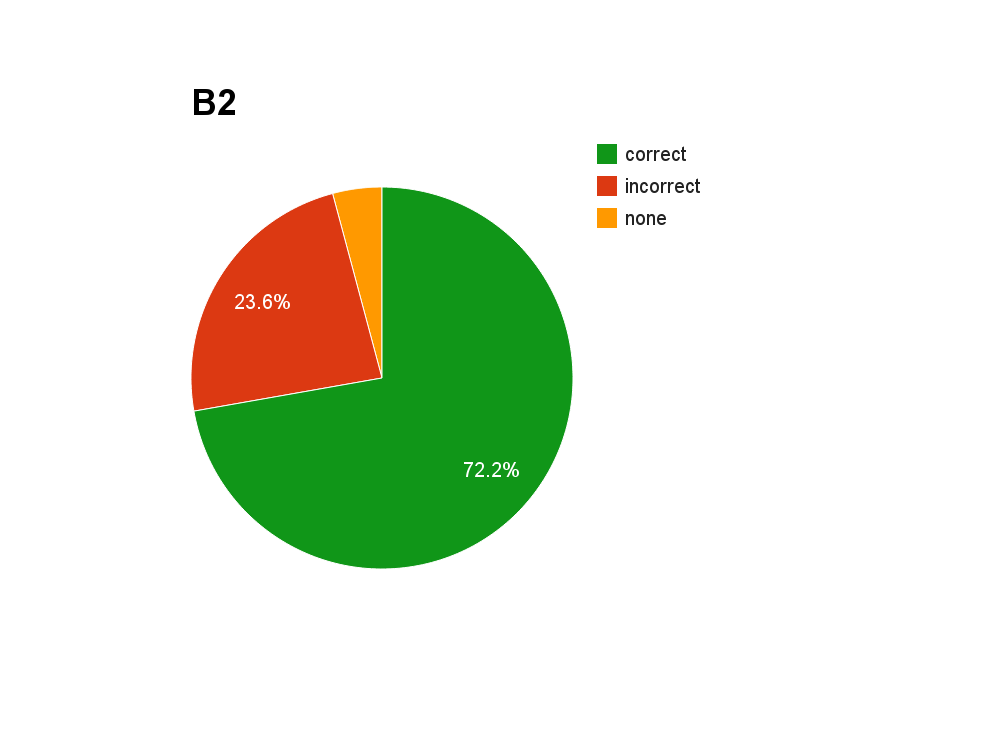
\includegraphics[width=\textwidth]{img/annotation/B2}
					\caption{B2}
					\label{fig:levelpies:B2}
				\end{subfigure}%
				~
				\begin{subfigure}[b]{0.5\textwidth}
					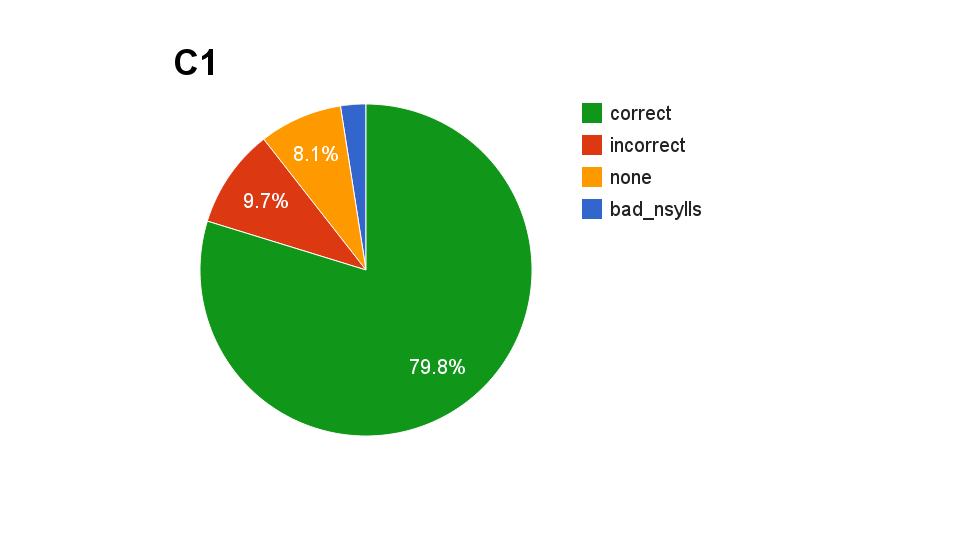
\includegraphics[width=\textwidth]{img/annotation/C1}
					\caption{C1}
					\label{fig:levelpies:C1}
				\end{subfigure}%
				\caption{\TODO{Caption}}
				\label{fig:levelpies}
			\end{figure}		
			
			
			
			\begin{figure}[htb]
				\centering
				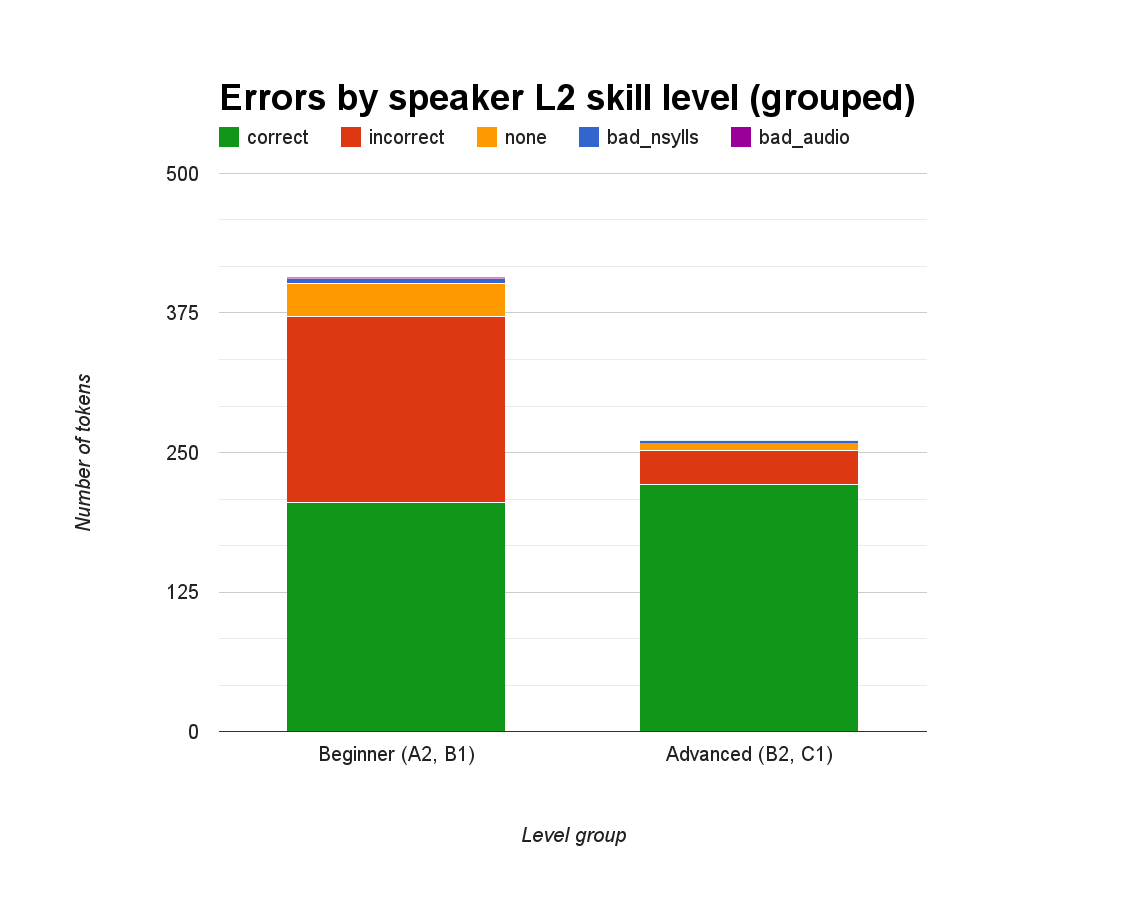
\includegraphics[width=\textwidth]{img/annotation/skillLevelGroupsBars}
				\caption{\TODO{Caption}}
				\label{fig:levelgroupsbars}
			\end{figure}
			
			
			\begin{figure}[htb]
				\centering
				\begin{subfigure}[t]{0.5\textwidth}
					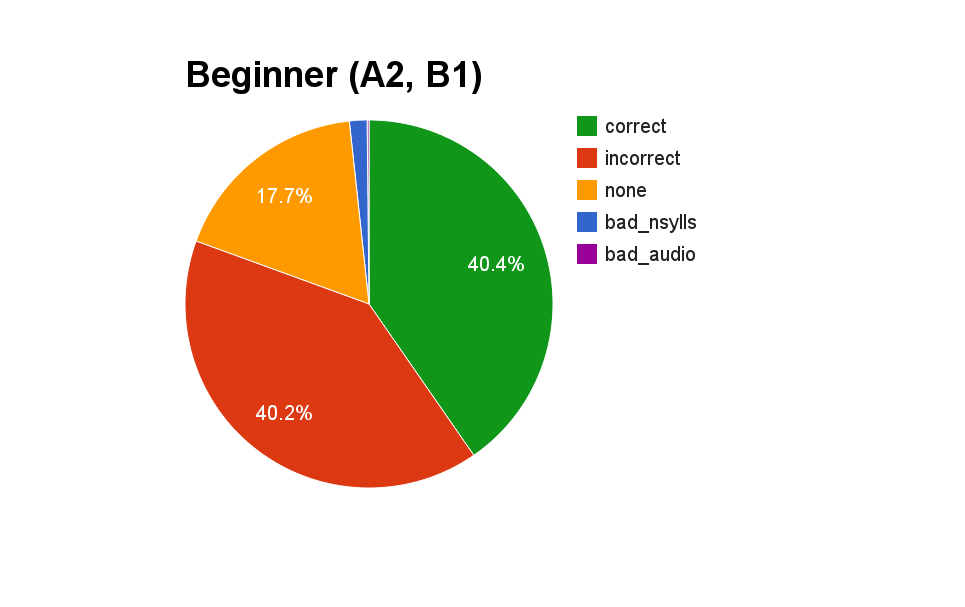
\includegraphics[width=\textwidth]{img/annotation/beginnerPie}
					\caption{}
					\label{fig:levelgroupspies:beg}
				\end{subfigure}%
				~
				\begin{subfigure}[t]{0.5\textwidth}
					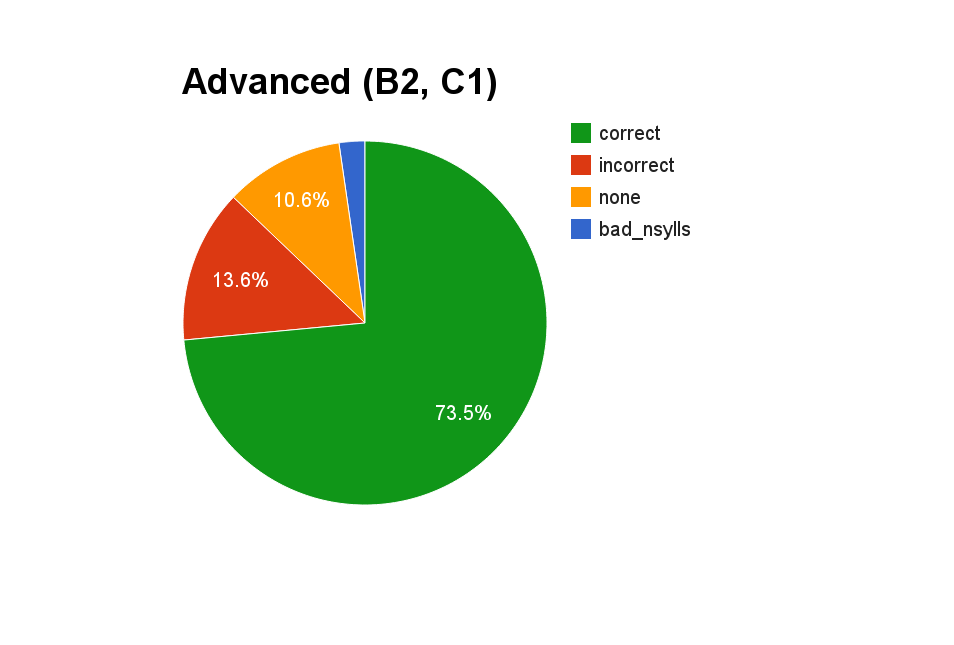
\includegraphics[width=\textwidth]{img/annotation/advancedPie}
					\caption{}
					\label{fig:levelgroupspies:adv}
				\end{subfigure}%
				\caption{\TODO{Caption}}
				\label{fig:levelgroupspies}
			\end{figure}	
			
		
		\subsection{Errors by speaker age and gender}
		\label{sec:results:agegender}
			\TODO{}
			
		
		\subsection{Errors by recording condition}
		\label{sec:results:condition}
			\TODO{}
		
		
		%\subsubsection{Accuracy by word type}
		\subsection{Errors by word type}
		\label{sec:results:wordtype}
			\TODO{}
	
		\subsection{Impact of technical problems}
		\label{sec:results:techproblems}
			\TODO{}
	
	
	\section{Summary}
	\label{sec:lexstress:summary}
	\TODO{}